% LaTex Template

\documentclass[12pt]{article}
%\usepackage{natbib}
\usepackage[letterpaper, margin=1.1in]{geometry}
\usepackage{graphicx}
\usepackage{wrapfig}
\usepackage{enumitem}
\setlist[enumerate]{itemsep=0mm}
\usepackage{multirow}
\usepackage[table,xcdraw]{xcolor}
\usepackage{lscape}
\usepackage{caption}
\usepackage{subcaption}

\begin{document}
\noindent{Alexandra Pulwicki \\ \today}

\begin{center}
\Large \textbf{Appendix\\ Variability}
\end{center}

Point Scale
- boxplots, std, 
Zigzag
- vertex vs measured, plots, variograms, mean + std + vario summary table
Watershed
- plots, variograms, mean + std + vario summary table


\subsection*{Point Scale}

\subsubsection*{Observer differences}

A one-way ANOVA for each transect pattern of snow depth measurements taken by different observers  shows that there are no differences between observers. The only exception is the Lower Hourglass on Glacier 4, where one observer had higher mean snow depth than the other two (p $<$ 0.05). This shows that observer bias is not present in this study and no corrections to the data based on observer were applied.

 The mean standard deviation of measurements taken at each location within various groups can be seen in Table \ref{tab:point_std}. The mean standard deviation varies between glaciers, patterns, and observers but overall, the reproducibility of depth measurement is on the order of centimetres. This is a small variability compared to the  

\begin{table}[]
\centering
\caption{Mean standard deviation (cm) of snow depth measurements for various groupings.}
\label{tab:point_std}
\begin{tabular}{cccccccc}
 &  &  &  & \multicolumn{4}{c}{\textbf{Person}} \\
\multirow{-2}{*}{\textbf{Glacier}} & \multirow{-2}{*}{\textbf{Pattern}} & \multirow{-2}{*}{\textbf{\begin{tabular}[c]{@{}c@{}}Overall \\ Glacier\end{tabular}}} & \multirow{-2}{*}{\textbf{\begin{tabular}[c]{@{}c@{}}Overall \\ Pattern\end{tabular}}} & AP & GF & CA & AC \\ \hline
\rowcolor[HTML]{EFEFEF} 
\cellcolor[HTML]{EFEFEF} & LH & \cellcolor[HTML]{EFEFEF} & 5.1 & 4.8 & - & 8.5 & 2 \\
\rowcolor[HTML]{EFEFEF} 
\cellcolor[HTML]{EFEFEF} & LC & \cellcolor[HTML]{EFEFEF} & 4.7 & 4.3 & - & 8.2 & 1.7 \\
\rowcolor[HTML]{EFEFEF} 
\cellcolor[HTML]{EFEFEF} & LM & \cellcolor[HTML]{EFEFEF} & 3.7 & - & 4.7 & 4.6 & 1.9 \\
\rowcolor[HTML]{EFEFEF} 
\cellcolor[HTML]{EFEFEF} & UH & \cellcolor[HTML]{EFEFEF} & 2.6 & 3.4 & 2.2 & - & 2.3 \\
\rowcolor[HTML]{EFEFEF} 
\cellcolor[HTML]{EFEFEF} & UC & \cellcolor[HTML]{EFEFEF} & 1.9 & 1.9 & 2.3 & - & 1.5 \\
\rowcolor[HTML]{EFEFEF} 
\cellcolor[HTML]{EFEFEF} & UM & \cellcolor[HTML]{EFEFEF} & 1.9 & - & 1.7 & 2 & 2 \\
\rowcolor[HTML]{EFEFEF} 
\multirow{-7}{*}{\cellcolor[HTML]{EFEFEF}G04} & UT & \multirow{-7}{*}{\cellcolor[HTML]{EFEFEF}3.5} & 3.9 & 3.7 & - & 2.4 & 5.6 \\
 & LH &  & 5.4 & 4.8 & - & 6.1 & - \\
 & LC &  & 5 & 3.9 & - & 6.2 & - \\
 & LM &  & 6.5 & - & 6.8 & 6.5 & 6 \\
 & UH &  & 4.1 & 3.5 & 4.4 & 4.5 & - \\
 & UC &  & 7 & 5.5 & 7 & 8.7 & - \\
 & UM &  & 4.2 & 3.2 & 5.2 & 4.1 & - \\
 & UT &  & 5.6 & 3.2 & - & 8.2 & - \\
\multirow{-8}{*}{G02} & BT & \multirow{-8}{*}{5.1} & 2.2 & 2.2 & - & 3 & 1.5 \\
\rowcolor[HTML]{EFEFEF} 
\cellcolor[HTML]{EFEFEF} & LH & \cellcolor[HTML]{EFEFEF} & 3.8 & 3.1 & 4.1 & 4 & - \\
\rowcolor[HTML]{EFEFEF} 
\cellcolor[HTML]{EFEFEF} & LC & \cellcolor[HTML]{EFEFEF} & 4.5 & 2.9 & 4.8 & 5.8 & - \\
\rowcolor[HTML]{EFEFEF} 
\cellcolor[HTML]{EFEFEF} & LM & \cellcolor[HTML]{EFEFEF} & 6.6 & 4.6 & 7.7 & 7.6 & - \\
\rowcolor[HTML]{EFEFEF} 
\cellcolor[HTML]{EFEFEF} & UH & \cellcolor[HTML]{EFEFEF} & 3.5 & 3.4 & 3.6 & 3.4 & - \\
\rowcolor[HTML]{EFEFEF} 
\cellcolor[HTML]{EFEFEF} & UC & \cellcolor[HTML]{EFEFEF} & 3.8 & 3.4 & 4 & 4 & - \\
\rowcolor[HTML]{EFEFEF} 
\cellcolor[HTML]{EFEFEF} & UM & \cellcolor[HTML]{EFEFEF} & 4.8 & 4.4 & 5.8 & 4.4 & - \\
\rowcolor[HTML]{EFEFEF} 
\multirow{-7}{*}{\cellcolor[HTML]{EFEFEF}G13} & UT & \multirow{-7}{*}{\cellcolor[HTML]{EFEFEF}4.2} & 4.1 & 2.7 & 4.8 & 4.6 & - \\
\end{tabular}
\end{table}


\begin{wrapfigure}{r}{0.75\textwidth} 
	\centering
	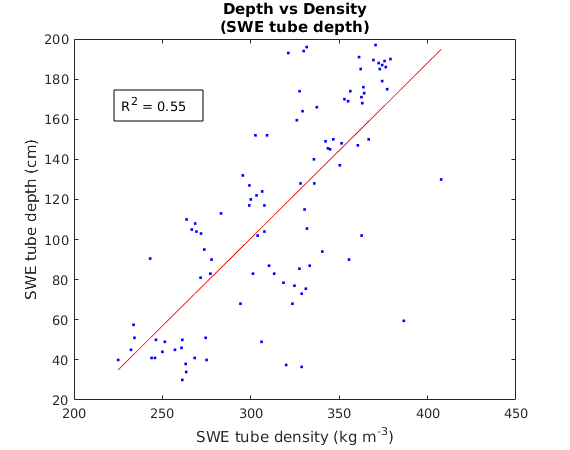
\includegraphics[width =0.75\textwidth]{DepthDensity_SWEtube.png}\\
	\caption{Relationship between measured density and snow depth for all Federal Sampler measurements.}
	\label{fig:tube_depth}
\end{wrapfigure}

\begin{enumerate}
\item 
\end{enumerate}










\end{document}